% vim: set spell spelllang=es syntax=tex :

\documentclass[11pt,a4paper,spanish]{beamer}

\usepackage[spanish]{babel}

\usepackage[utf8]{inputenc}

\usepackage{graphicx}

\usepackage{subcaption} %Para Subfigure

\usepackage{caption} %Para captions en las figuras sin prefijo

\usepackage{ccicons}

\usepackage{url}

\usepackage{babelbib}

\usepackage{textcomp}

\usepackage{tabularx}

\usepackage{styles/egyptian}

\newcommand{\aprox}{\raisebox{0.5ex}{\texttildelow}}
\newcommand{\bit}{\textbf{b}}
\newcommand{\Byte}{\textbf{B}}

\newcommand{\multiline}[2][c]{
      \begin{tabular}[#1]{@{}c@{}}#2\end{tabular}
      }


\usefonttheme{serif}

\setlength{\parskip}{1.5mm}

\usetheme{Rochester}
\usecolortheme{whale}

%\usetheme{Warsaw}

\beamertemplatenavigationsymbolsempty

\setbeamertemplate{background canvas}{
    \raisebox{-0.99\paperheight}[0pt][0pt]{
        \makebox[\paperwidth]{
            \null
            \hspace{-1em}
            \includegraphics[width=0.09\paperwidth]{logos/fai.pdf}
            \hspace{0.8\paperwidth}
            \hspace{-0.5em}
            \includegraphics[width=0.09\paperwidth]{logos/uncoma.pdf}
            }
    }
}

\defbeamertemplate{footline}{centered page number}
{
    \hspace*{\fill}
    \usebeamercolor[fg]{blue}
    \usebeamerfont{page number in head/foot}
    \insertpagenumber\,/\,\insertpresentationendpage
    \hspace*{\fill}\vskip2pt
}
\setbeamertemplate{footline}[centered page number]

\title{Organización y Arquitectura de computadoras}
\author{}
\date{}

\begin{document}

\begin{frame}[noframenumbering]


    \maketitle
    \centering
    %\vspace{-8em}~
    %\begin{figure}
    %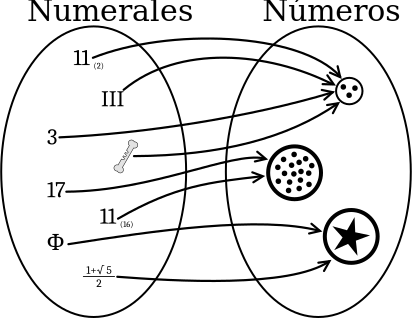
\includegraphics[height=0.65\textheight]{img/numerales.pdf}
        %\captionsetup{textfont=tiny,labelformat=empty,justification=centering}
        %\caption{}
    %\end{figure}

\end{frame}

\begin{frame}

    \frametitle{Temario}

\begin{itemize}

    \item Componentes básicos de una computadora:
    \begin{itemize}
        \item \emph{¿¿??}
        \item \emph{¿¿??}
        \item \emph{¿¿??}
        \item \emph{¿¿??}
        \item Arquitectura de Von Neumann.
        \item \emph{¿¿??}
        \item Caso de estudio
            \begin{itemize}
                \item Modelo Computacional Binario Elemental (MCBE).
            \end{itemize}
    \end{itemize}

\end{itemize}
\end{frame}

\begin{frame}
    \frametitle{Componentes básicos de una computadora}
    \begin{itemize}
        \pause
        \item Memoria.
        \pause
        \item CPU.
        \pause
        \item Dispositivos de entrada/salida.
        \pause
        \item Buses.
    \end{itemize}
\end{frame}

\begin{frame}
    \frametitle{Componentes básicos de una computadora}
    \framesubtitle{Memoria (Memoria principal)}
    \pause
    \begin{itemize}
        \item Normalmente implementada con circuitos \textbf{biestables}, cada
            uno almacenando un \textbf{bit}. \pause
        \item Los \textbf{bits} se agrupan en \textbf{bytes}.
            \pause
        \item La memoria se divide celdas de un \textbf{byte}, cada una con su
            propia dirección numerada de $0$ a $n-1$. \pause
        \item Puede contener \emph{datos} o \emph{instrucciones}.
    \end{itemize}
\end{frame}

\begin{frame}
    \frametitle{Componentes básicos de una computadora}
    \framesubtitle{CPU: Unidad Central de Procesamiento}
    \pause
    \begin{itemize}
        \item Interpreta y ejecuta un conjunto de instrucciones almacenados en
            la memoria. \pause
        \item Circuito secuencial. \pause
        \item Contiene registros. \pause
        \item Organización de la CPU: \pause
        \begin{itemize}
            \item CU: Unidad de control. \pause
            \item ALU: Unidad Aritmético-Lógica. \pause
            \item Registros. \pause
            \item Buses internos.
        \end{itemize}
    \end{itemize}
\end{frame}

\begin{frame}
    \frametitle{Arquitectura y Organización}
    \begin{itemize}
        \item \emph{Arquitectura de computadoras}: Es el diseño conceptual de
            la estructura y componentes desde el punto de vista funcional.
        \item \emph{Organización de computadoras}: Es la descripción de la
            implementación especifica.
    \end{itemize}
\end{frame}

\begin{frame}
    \frametitle{Componentes básicos de una computadora}
    \framesubtitle{Dispositivos de entrada/salida (E/S)}
    \pause
    \begin{itemize}
        \item Dispositivos que permiten a la computadora comunicarse con el
            mundo exterior. \pause
        \item Pueden exclusivamente de entrada, exclusivamente de salida, o
            realizar ambas tareas. \pause
        \item Ejemplos:
        \begin{itemize}
            \item Entrada: Teclado, mouse, giroscopios, cámara.
            \item Salida: Pantalla, parlantes.
            \item Entrada y salida: Placa de red, Discos duros, pendrives.
        \end{itemize}
    \end{itemize}
\end{frame}

\begin{frame}
    \frametitle{Componentes básicos de una computadora}
    \framesubtitle{Buses}
    \pause
    \begin{itemize}
        \item Interconexión entre componentes:\pause
        \begin{itemize}
            \item \emph{Buses de sistema}: Interconectan la CPU y memoria.
            \item \emph{Buses internos}: Interconectan los componentes de la
                CPU.
            \item \emph{Buses de Entrada/Salida}: Interconectan al sistema con
                los dispositivos de \emph{E/S}.
        \end{itemize}
    \end{itemize}
\end{frame}

\begin{frame}
    \frametitle{Componentes básicos de una computadora}
    \centering
    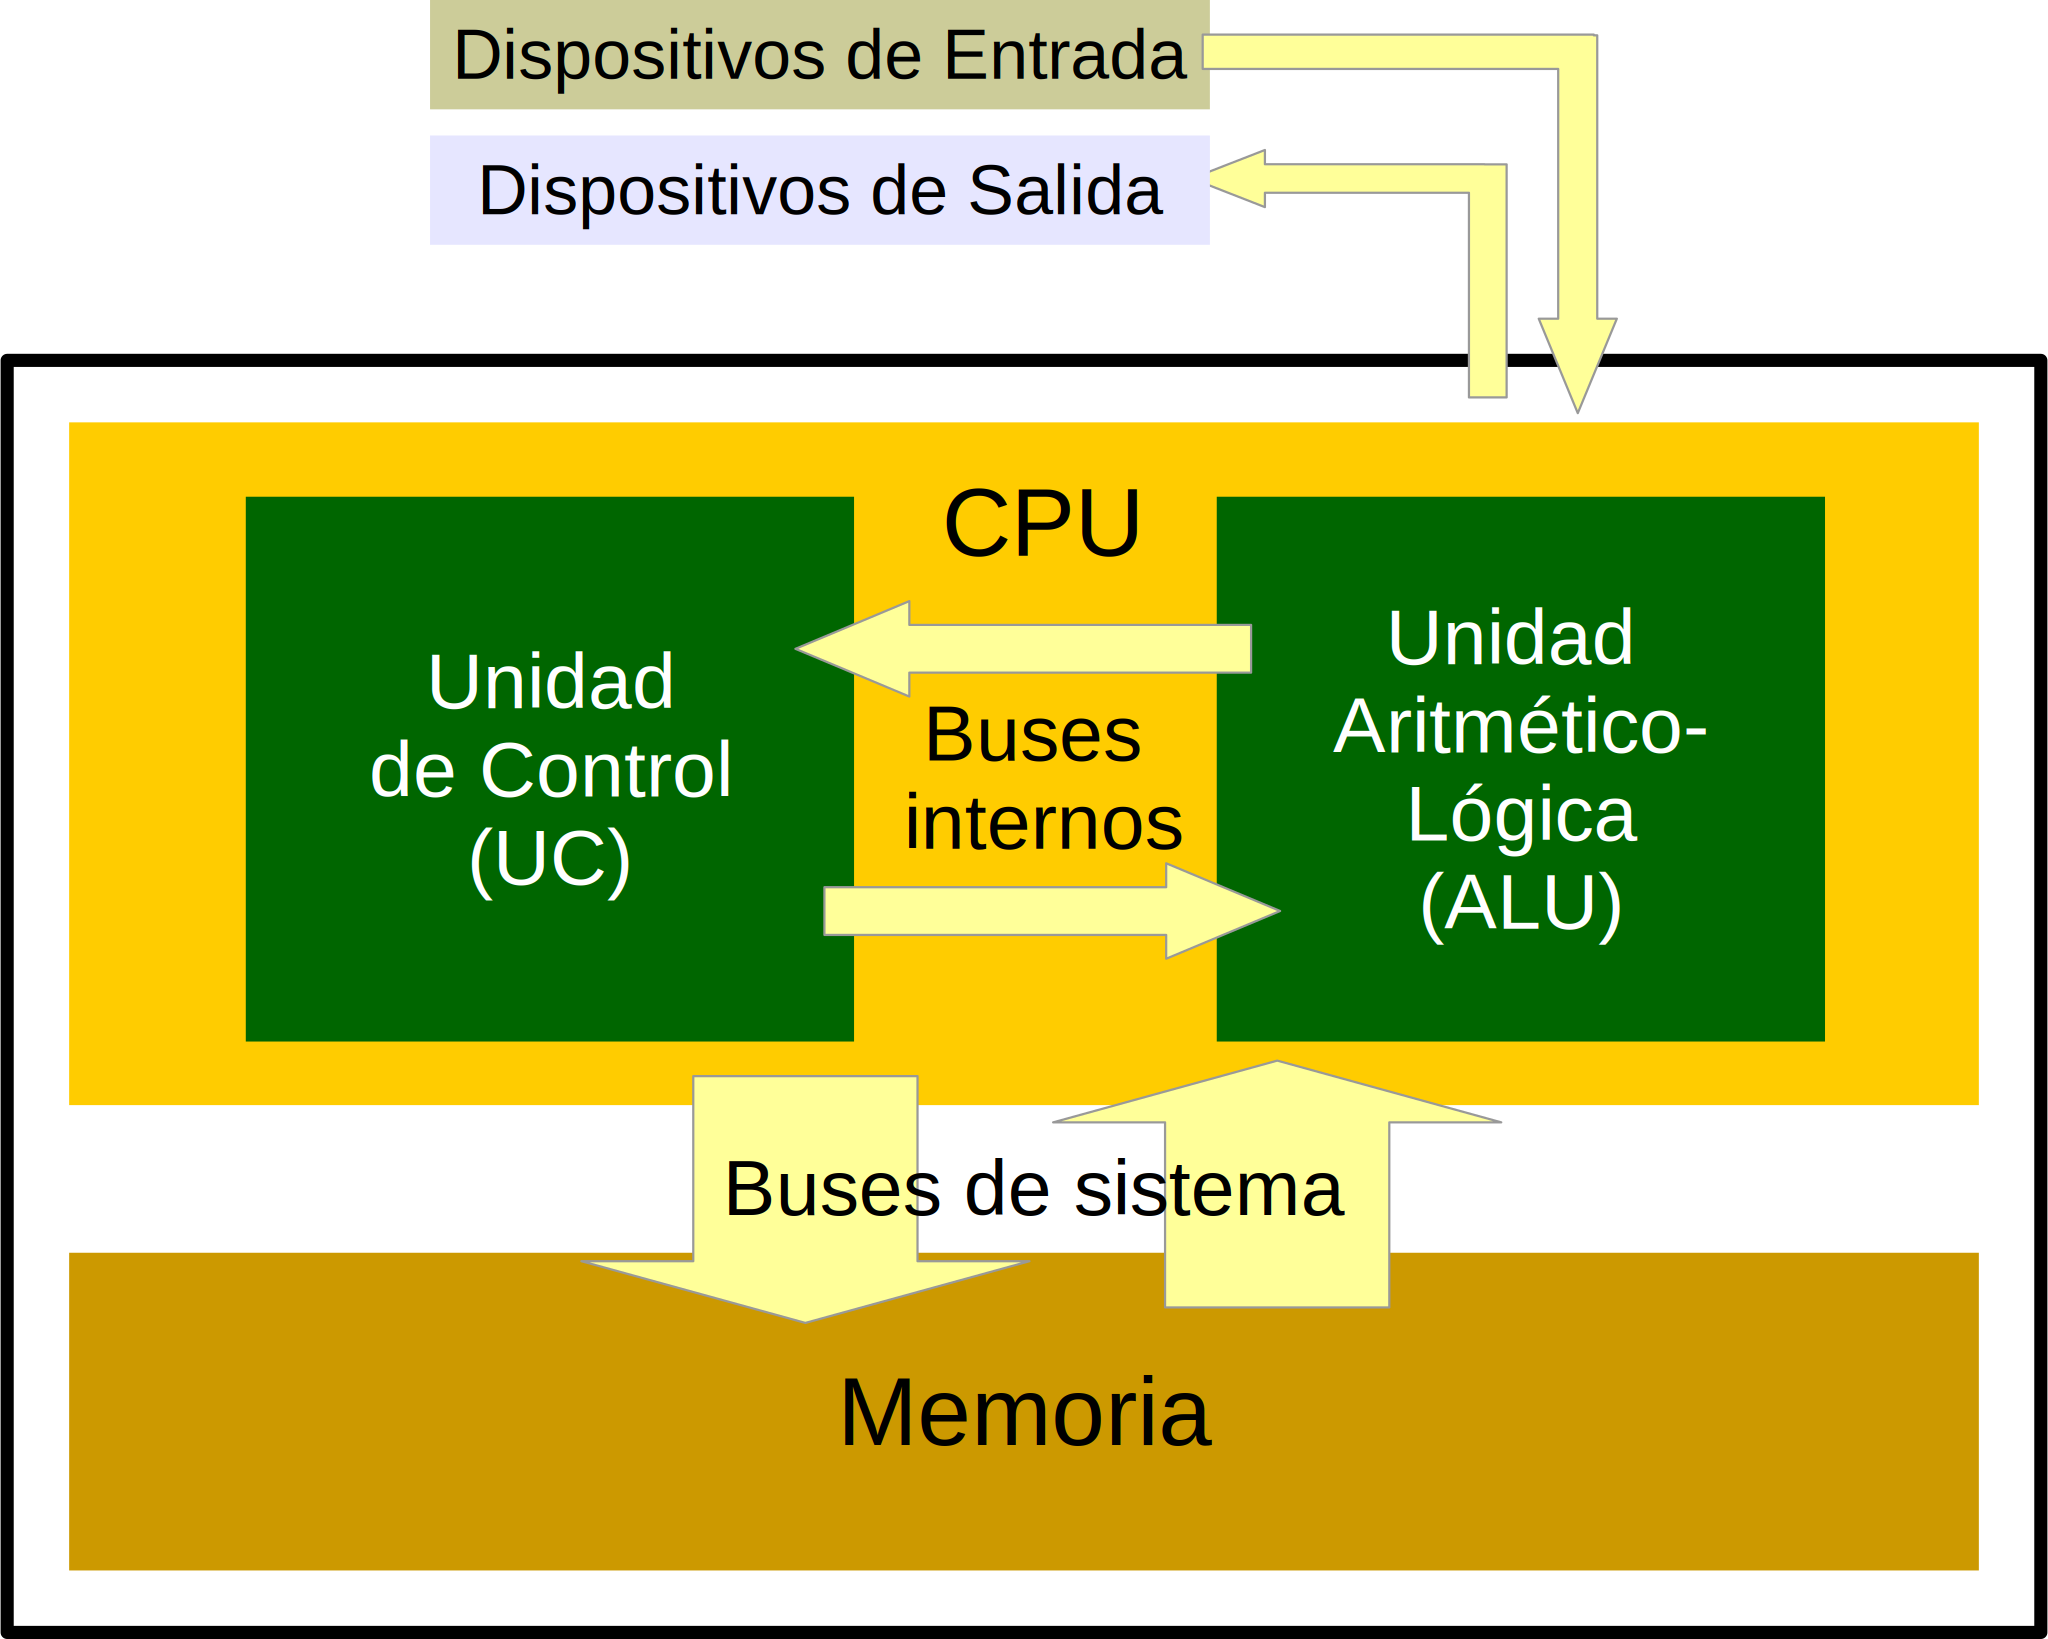
\includegraphics[height=0.9\textheight]{img/arquitecturaComp.pdf}
\end{frame}

\begin{frame}
    \frametitle{Componentes básicos de una computadora}
    \framesubtitle{Arquitectura de Von Neumann}
    \pause
    \begin{itemize}
        \item Arquitectura de programa almacenado. \pause
        \item Datos e instrucciones se almacenan en la misma memoria. \pause
        \item La ejecución de un programa es secuencial (hacia direcciones
            ascendentes) salvo que aparezcan instrucciones de transferencia de
            control (saltos).
    \end{itemize}
\end{frame}

\begin{frame}
    \frametitle{Componentes básicos de una computadora}
    \framesubtitle{ISA (Instruction set architecture): conjunto de
    instrucciones}
    \pause
    \begin{itemize}
        \item Conjunto de instrucciones que ejecuta la CPU. \pause
        \item Las instrucciones máquina son códigos binarios, de los cuales la
            \emph{CU} decodifica el código de operación y los parámetros.
            \pause
        \item Dos computadoras pueden compartir el mismo conjunto de
            instrucciones y arquitectura, pero tener distinta organización.
            \pause
        \item Hay arquitecturas donde todas las instrucciones tienen el mismo
            tamaño (en bits), otras de tamaño variable.
    \end{itemize}
\end{frame}

\begin{frame}
    \frametitle{Arquitectura de Von Neumann}
    \framesubtitle{Ciclo de instrucción}

    \begin{itemize}
        \item La CPU contiene como mínimo 2 registros:
        \begin{itemize}
            \item \emph{PC}: Contador de programa, contiene la dirección de la
                próxima instrucción a ejecutar.
            \item \emph{IR}: Donde se almacena la instrucción a ejecutar.
        \end{itemize}
    \end{itemize}
    \pause
    \begin{enumerate}
        \item La CPU recupera de la memoria el dato almacenado en la dirección
            indicada por el registro \textbf{PC} y lo almacena en el registro
            IR.  \pause
        \item La \emph{Unidad de Control} decodifica la instrucción almacenada
            en el registro IR. \pause
        \item Se ejecuta la instrucción. El \textbf{PC} se modifica de manera
            acorde.  \pause
        \item Se vuelve a ejecutar el primer paso. \pause
    \end{enumerate}
\end{frame}

\begin{frame}
    \frametitle{Caso de estudio}
    \framesubtitle{Modelo Computacional Binario Elemental (MCBE)}
    \begin{itemize}
        \item Tres registros de 8 bits: \textbf{PC}, \textbf{IR} y \textbf{AC}
            (acumulador).
        \item 32 celdas de memoria de 8 bits.
        \item Las celda 30 esta mapeada a entrada, y la 31 a salida.
        \item 8 instrucciones de 8 bits:
            \begin{itemize}
                \item 3 bits para el código de operación.
                \item 5 para indicar el operando.
            \end{itemize}
        \item Todos los registros y la memoria que no esta especificada
            comienza en cero.
    \end{itemize}
\end{frame}

\begin{frame}
    \frametitle{Modelo Computacional Binario Elemental (MCBE)}
    \framesubtitle{Instrucciones}

\tiny
\begin{tabularx}{\textwidth}{c|c|X}

    \textbf{Código de} & \textbf{Operando} &
    \multicolumn{1}{c}{\textbf{Descripción}} \\

    \textbf{operación} & & \\

    \emph{3 bits} & \emph{5 bits} & \\
    \hline
    \hline

    010 & \emph{dirección} & \textbf{Memoria → Acumulador}. Copia un byte
    desde la dirección de memoria al acumulador. El \textbf{PC} se incrementa
    en 1.\\ \hline

    011 & \emph{dirección} & \textbf{Acumulador → Memoria}. Copia el contenido
    del acumulador en esa dirección de memoria. El \textbf{PC} se incrementa
    en 1.\\ \hline

    100 & \emph{dirección} & \textbf{Suma}. El contenido de la dirección se
    suma al acumulador, y el resultado se almacena en el acumulador. El
    \textbf{PC} se incrementa en 1.\\ \hline

    101 & \emph{dirección} & \textbf{Resta}. El contenido de la dirección se
    resta al acumulador, y el resultado se almacena en el acumulador. El
    \textbf{PC} se incrementa en 1.\\ \hline

    110 & \emph{desplazamiento} & \textbf{Salto incondicional}. Se
    suma (en complemento a 2) el desplazamiento al \textbf{PC}. \\ \hline

    111 & \emph{desplazamiento} & \textbf{Salto condicional}. Si
    el acumulador es cero, se suma (en complemento a 2) el desplazamiento al
    \textbf{PC}, en caso contrario el \textbf{PC} se incrementa en uno. \\
    \hline

    001 & \emph{(sin uso)} & \textbf{Detiene la maquina}. No se
    ejecutan nuevas instrucciones. Los registros y la memoria quedan con el
    último valor que tenían. \\ \hline

    000 & \emph{(sin uso)} & \textbf{No operación}. No tiene
    ningún efecto sobre el acumulador ni memoria. El \textbf{PC} se incremente
    en uno. \\

\end{tabularx}
\end{frame}

\begin{frame}

    \frametitle{Modelo Computacional Binario Elemental (MCBE)}
    \framesubtitle{Ejemplo: programa}
    \centering
    \begin{tabular}{| c | c |}
        \hline
        \textbf{Dirección}&\textbf{Contenido binario}\\
        \hline \hline
        0 & 01000111 \\
        \hline
        1 & 01111111 \\
        \hline
        2 & 10001000 \\
        \hline
        3 & 01100111 \\
        \hline
        4 & 11100010 \\
        \hline
        5 & 11011011 \\
        \hline
        6 & 00100000 \\
        \hline
        7 & 00000010 \\
        \hline
        8 & 11111111 \\
        \hline
        \hline
\end{tabular}

\end{frame}

\begin{frame}

    \frametitle{Modelo Computacional Binario Elemental (MCBE)}
    \framesubtitle{Ejemplo: traza}
    \centering
    \resizebox{\textwidth}{!}{ \tiny
    \begin{tabular}{|c|c||c|c||c|c|c|c|}
        \hline
        \multicolumn{2}{|c||}{\multiline{Búsqueda de la \\
        instrucción }} &
        \multicolumn{2}{c||}{\multiline{Decodificación de la \\
        instrucción}} &
        \multicolumn{4}{c|}{Ejecución de la instrucción}\\
        \hline
        PC & IR & Cod. Op. & Operando & Acumulador & Memoria &
        Salida & PC \\
        \hline
        00000000  \pause &
        01000111 \pause &
        010 & 00111 \pause &
        00000010 & - & - & 00000001 \pause \\
        \hline
        00000001  \pause &
        01111111 \pause &
        011 & 11111 \pause &
        - & - & 00000010 & 00000010 \pause \\
        \hline
        00000010  \pause &
        10001000 \pause &
        100 & 01000 \pause &
        00000001 & - & - & 00000011 \pause \\
        \hline
        00000011  \pause &
        01100111 \pause &
        011 & 00111 \pause &
        - & (00000111)←00000001 & - & 00000100 \pause \\
        \hline
        00000100  \pause &
        11100010 \pause &
        111 & 00010 \pause &
        - & - & - & 00000101 \pause \\
        \hline
        00000101  \pause &
        11011011 \pause &
        110 & 11011 \pause &
        - & - & - & 00000000 \pause \\
        \hline
        00000000  \pause &
        01000111 \pause &
        010 & 00111 \pause &
        00000001 & - & - & 00000001 \pause \\
        \hline
        00000001  \pause &
        01111111 \pause &
        011 & 11111 \pause &
        - & - & 00000001 & 00000010 \pause \\
        \hline
        00000010  \pause &
        10001000 \pause &
        100 & 01000 \pause &
        00000000 & - & - & 00000011 \pause \\
        \hline
        00000011  \pause &
        01100111 \pause &
        011 & 00111 \pause &
        - & (00000111)←00000000 & - & 00000100 \pause \\
        \hline
        00000100  \pause &
        11100010 \pause &
        111 & 00010 \pause &
        - & - & - & 00000110 \pause \\
        \hline
        00000110  \pause &
        00100000 \pause &
        001 & 00000 \pause &
        - & - & - & -\\
        \hline
    \end{tabular}
    }

\end{frame}

\begin{frame}

    \frametitle{Temario}

\begin{itemize}

    \item Componentes básicos de una computadora:
    \begin{itemize}
        \item Memoria.
        \item CPU.
        \begin{itemize}
            \item Organización de la CPU.
        \end{itemize}
        \item Dispositivos de entrada/salida.
        \item Buses.
        \item Arquitectura de Von Neumann.
        \item Instrucciones y ejecución de instrucciones.
        \item Caso de estudio
            \begin{itemize}
                \item Modelo Computacional Binario Elemental (MCBE).
            \end{itemize}
    \end{itemize}

\end{itemize}
\end{frame}

\begin{frame}

\title{¿Consultas?}
\maketitle

\end{frame}

\newcounter{lastPage}
\setcounter{lastPage}{\number\value{page}}

\setcounter{page}{\number\value{lastPage}}

\end{document}
